\section{Neuronale Netzwerke} \label{ch:neural_networks}

Wie bereits erwähnt, hat sich der Name Neuronales Netzwerk durchgesetzt, obwohl es weder neuronal noch ein Netzwerk ist.
Sie werden verwendet, um komplexere Zuordnungen zu erstellen als die bisherigen Modelle in der Lage waren.
Im Folgenden wird erörtert, was die Motivation hinter diesem Konzept ist und wie Netzwerke trainiert werden.

\subsection{Deep Learning} \label{ch:deep_learning}

Auch wenn das universelle Approximationstheorem zeigt, dass alle kontinuierlichen Funktionen mit nur einer Schicht beschrieben werden können, ist es in der Praxis viel sinnvoller, mehrere Schichten zu unserem Modell hinzuzufügen, um die erforderlichen Ressourcen gering zu halten.
Rolnick und Tegmark \cite{Rolnick2017} zeigen, dass bei einschichtigen Modellen die Anzahl der Neuronen exponentiell mit der Anzahl der Variablen des Inputs wächst, während mehrschichtige neuronale Netzwerke lediglich linear wachsen.

\begin{figure}
    \centering
    \caption[Neuronales Netzwerk]{ Ein neuronales Netzwerk mit drei Eingangsknoten, zwei verborgenen Schichten mit je fünf Knoten und einer Ausgangsschicht mit drei Knoten. Der Bias wird jeder Schicht hinzugefügt, indem ein Knoten mit dem Wert eins vorangestellt wird. Jeder Knoten wird, wie im vorigen Beispiel, durch die Summe des Produkts der vorherigen Schicht und ihres jeweiligen Gewichts berechnet. }
    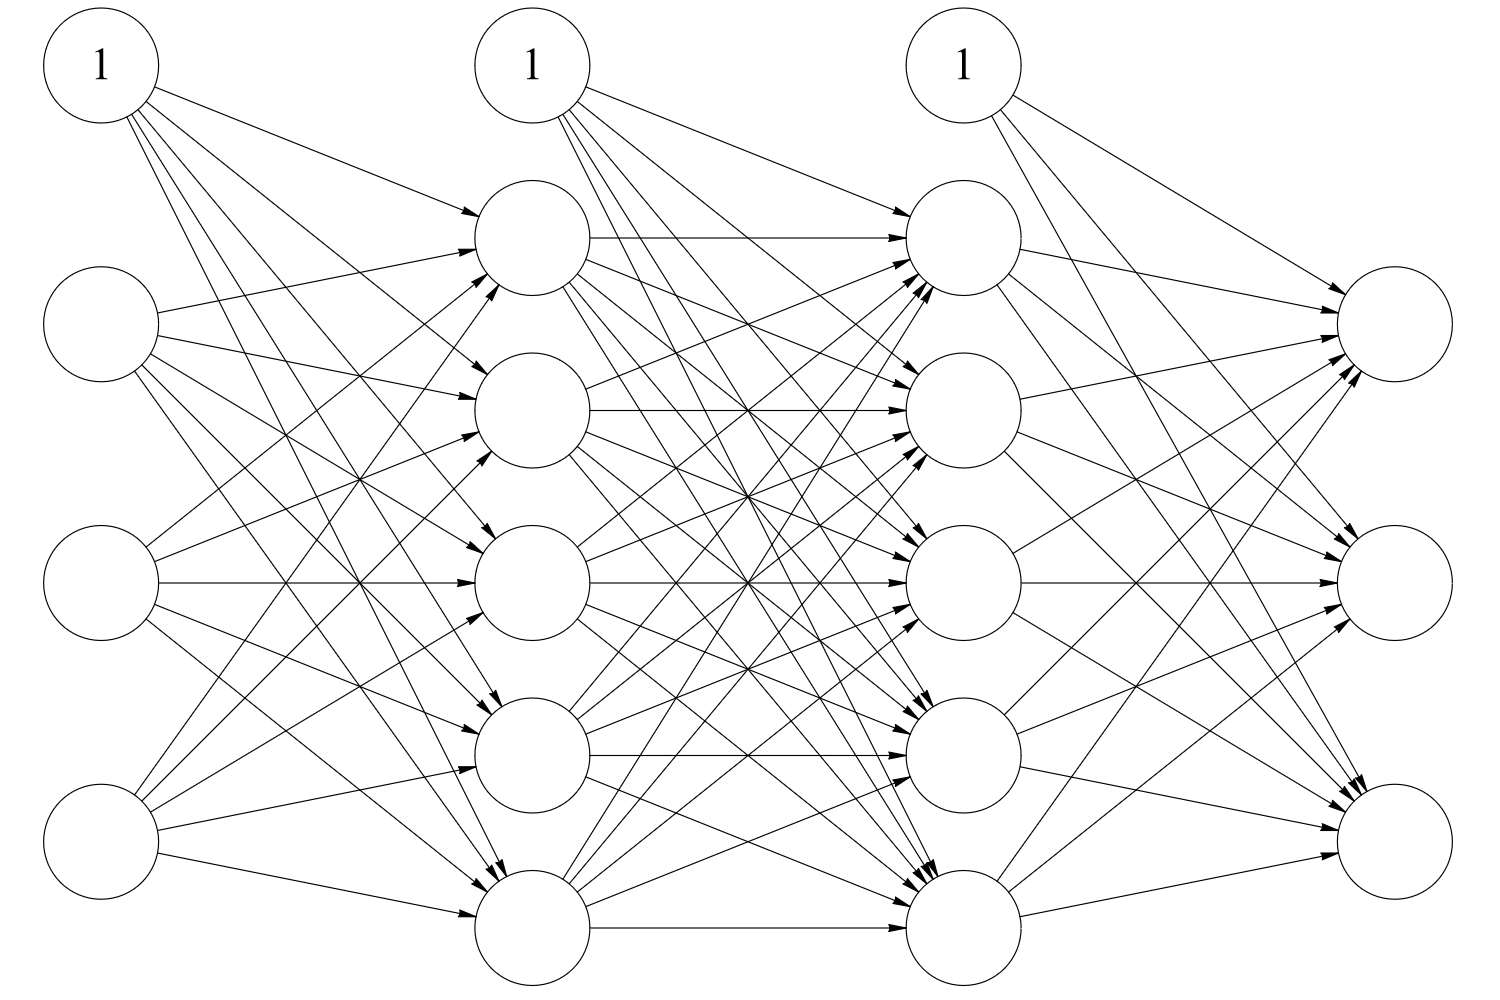
\includegraphics[width=0.6\textwidth]{images/2_nn_with_bias.png}
    \label{fig:nn}
\end{figure}

Jeder Knoten in Abbildung~\ref{fig:nn} kann durch die Notation $z^l_i$ angesprochen werden.
$l$ ist die Nummer der Schicht, in welcher der Knoten liegt, und $i$ ist der Index des Knotens.
Jedes Gewicht $\theta^l_{i, j}$ kann ebenfalls adressiert werden; $l$ ist die Schicht, auf welche die Gewichtung verweist, $i$ ist der Index des Knotens, der mit der Gewichtung multipliziert wird, um den Wert des Knotens in der Schicht $l$ mit dem Index $j$ zu beeinflussen.
So können wir jeden Knoten als Resultat folgender Gleichung beschreiben\footnote{In der Literatur wird der Bias oft separat hinzugefügt.
Gemäß der Konvention, dem Eingangsvektor $x$ eine 1 voranzustellen, wird er immer als Index 0 jeder Ebene aufgenommen.
Bitte beachten Sie, dass dies mathematisch gesehen dasselbe ist.}:

\begin{equation}
    z^l_j = \sum^n_{i=0}z^{l-1}_i\theta^l_{i, j}
    \label{eq:node_value}
\end{equation}

$n$ ist die Anzahl der Knoten in der jeweiligen Schicht. Gleichung~\eqref{eq:node_value} kann vektorisiert werden zu:

\begin{equation}
    z^l = \theta^l z^{l-1}
    \label{eq:node_value_vectorized}
\end{equation}

\subsection{Aktivierungsfunktionen}

Ein Problem bei den Werten der einzelnen Zellen ist, dass sie in beliebiger Größe erfolgen können. Numerisch gesehen ist dies sehr schwer zu kontrollieren, so dass die Knoten selbst wiederum zuerst an eine andere Funktion gegeben werden; diese Funktion wird passenderweise als Aktivierungsfunktion bezeichnet.


\begin{figure}
    \centering
    \begin{subfigure}[b]{0.3\textwidth}
        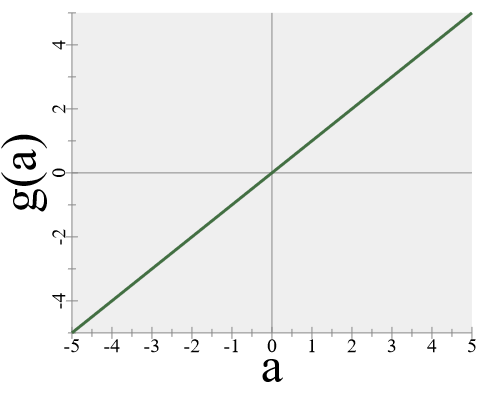
\includegraphics[width=\textwidth]{images/4_linear.png}
        \caption{Linear}
        \label{fig:activation_linear}
    \end{subfigure}
    \begin{subfigure}[b]{0.3\textwidth}
        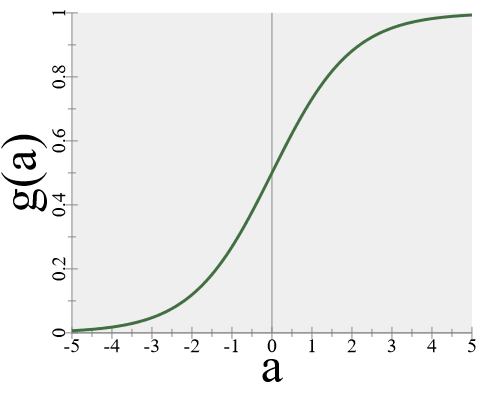
\includegraphics[width=\textwidth]{images/4_sigmoid.png}
        \caption{Logistischer Sigmoid}
        \label{fig:activation_sigmoid}
    \end{subfigure}
    \begin{subfigure}[b]{0.3\textwidth}
        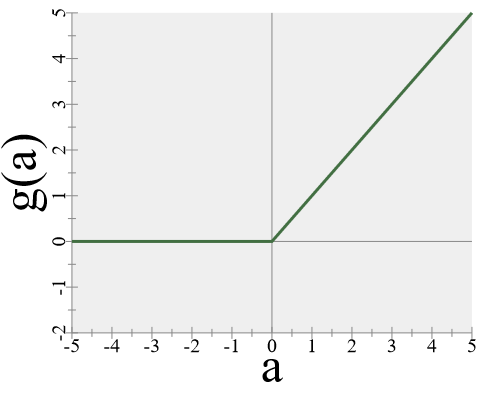
\includegraphics[width=\textwidth]{images/4_relu.png}
        \caption{ReLU}
        \label{fig:activation_relu}
    \end{subfigure}
    \caption{Aktivierungsfunktionen} % TODO maybe add some text to activation functions?
    \label{fig:activation}
\end{figure}

Die Aktivierungsfunktionen werden auf unterschiedliche Weise genutzt und bieten weitere Möglichkeiten der Anpassung durch weitere Parameter, um die Modellleistung zu erhöhen.
Bisher wurde die in Abbildung~\ref{fig:activation_linear} gezeigte lineare Funktion mit der Abbildung $g(a) = a$ angenommen, in welcher der Eingang und Ausgang äquivalent sind.
Der logistische Sigmoid wird in der Praxis oft verwendet, da es beliebige Eingaben in das Intervall $[0,1]$ verteilt.
Die "rectified linear unit" (ReLU) ist rechnerisch erheblich simpler und wird für die Verwendung mit den meisten vorwärts gerichteten neuronalen Netzen \cite[S.169]{Goodfellow2017}\cite{Glorot2011} empfohlen.
Mathematische Darstellungen werden in den Gleichungen~\eqref{eq:sigmoid_relu} gezeigt.

\begin{equation}
    \begin{split}
        Sigmoid: f(x) & = \frac{1}{1 + \exp^{-x}} \\ ReLU: f(x) & = max(0, x)
    \end{split}
    \label{eq:sigmoid_relu}
\end{equation}

Die Verwendung der Aktivierungsfunktionen kann ebenfalls variieren; z.B. ist es üblich, dass das logistische Sigmoid einen Schwellenwert hat, um überhaupt nicht zu feuern, wenn ein bestimmter Wert (z.B. 0,5) nicht erreicht wird.

Durch die Einführung von Aktivierungsfunktionen belaufen sich die Gleichungen~\eqref{eq:node_value} und \eqref{eq:node_value_vectorized} zu:

\begin{equation}
    a^l_j = \sigma(z^l_j) = \sigma(\sum^n_{i=0}z^{l-1}_i\theta^l_{i, j})
    \label{eq:activation}
\end{equation}

Mit der entsprechenden vektorisierten Gleichung:

\begin{equation}
    a^l = \sigma(z^l) = \sigma(\theta^l z^{l-1})
    \label{eq:activation_vectorized}
\end{equation}

Es gibt eine Vielzahl verschiedener Aktivierungsfunktionen, wobei diese beiden am prominentesten sind.
Die Auswahl der Aktivierungsfunktion und eventuell ein entsprechender Schwellenwert sind ein weiterer Hyperparameter, der vor dem Training gewählt werden muss.

\subsection{Backpropagation}

Beim Gradientenabstieg~\eqref{eq:gradient_descent} können nicht alle Parameter in allen Ebenen aktualisiert werden, da er nur die Aktualisierung der Parameter der letzten Ebene berücksichtigt, wenn sie als unabhängig vorangegangener Ebenen betrachtet wird.
Da die letzte Schicht eine Funktion der jeweils vorhergehenden Schicht ist, kann die Kettenregel angewendet werden und so der berechneten Fehler der letzten Schicht auf die Vorangegangene übertragen und die Gewichte bzw. den Bias aktualisieren. Dieser Umstand gilt für jede Schicht, mit Ausnahme der Eingangsschicht (die schließlich nicht aktualisiert werden muss).
Die folgenden Gleichungen wurden mit \cite[S.733]{StuartRussell2018}, \cite[S.197]{Goodfellow2017} und \cite[ch.2]{Nielsen2015} zusammengestellt:

\begin{equation}
    \varDelta^L = \nabla_a L \odot \sigma'(z^L)
    \label{eq:output_error}
\end{equation}
\begin{equation}
    \varDelta^l = ((\theta^{l+1})^T \varDelta^{l+1}) \odot \sigma'(z^l)
    \label{eq:hidden_error}
\end{equation}
\begin{equation}
    \theta_{i+1} := \theta_i - \eta \varDelta
    \label{eq:backprop_update}
\end{equation}

Gleichung~\eqref{eq:output_error} beschreibt den in der Ausgabeschicht berechneten Fehler. Wir definieren unser Netzwerk mit $L$-Schichten, daher wird die Ausgabeschicht immer durch den Index $L$ beschrieben.
$\odot$ ist der Hadamard-Operator. Er wird verwendet, um Tensoren elementweise zu multiplizieren, was in diesem Fall nützlich ist, da er verhindert, dass die Vektoren in Diagonalmatrizen transformiert werden müssen.
Gleichung~\eqref{eq:output_error} ist ein direktes Ergebnis der Anwendung der multivariaten Kettenregel auf die Ableitung der in der letzten Schicht durchgeführten Verlustfunktion.
Wie bereits erwähnt wird der Gradientenabstieg durch die Ableitung der Verlustfunktion in Gleichung~\eqref{eq:sgd_mse_here} durchgeführt.
Da zwischen dem in der Verlustfunktion verwendeten Eingang und dem Ausgang der vorhergehenden Schicht eine Aktivierungsfunktion implementiert ist, muss die Kettenregel auch auf diese angewendet werden.

\begin{equation}
    \frac{\partial L}{\partial z^L_j} = \frac{\partial L}{\partial a^L_j}\frac{\partial a^L_j}{\partial z^L_j}
    \label{eq:proof_loss_chain_rule}
\end{equation}

Indem man darauf hinweist, dass $\frac{\partial L}{\partial a^L_i}$ nur eine nicht vektorisierte Form von $\nabla_a L$ und $\frac{\partial a^L_i}{\partial z^L_i}$ von $\sigma'(z^L)$ ist, wird die Äquivalenz deutlich.

Gleichung~\eqref{eq:hidden_error} kann folgendermaßen umgeschrieben werden:

\begin{equation}
    \varDelta^l_i = \frac{\partial L}{\partial z^l_i} = \sum_{j=0}^n (\frac{\partial L}{\partial z^{l+1}_j}\frac{\partial z^{l+1}_j}{\partial z^l_i})
\end{equation}

$n$ ist die Anzahl der Knoten in der nachfolgenden Schicht. Aus $\frac{\partial L}{\partial z^{l+1}_i} = \varDelta^{l+1}_i$ folgt:

\begin{equation}
    \frac{\partial L}{\partial z^l_i} = \sum_{j=0}^n (\varDelta^{l+1}_j \frac{\partial z^{l+1}_j}{\partial z^{l}_i})
    \label{eq:hidden_error_intermediate}
\end{equation}

Die folgende Gleichung ist ebenfalls bekannt:

\begin{equation}
    \begin{split}
    z^{l+1}_j & = \sum_{i=0}^n \theta^{l+1}_{i,j} a^l_i = \sum_{i=0}^n \theta^{l+1}_{i, j} \sigma(z^l_i) \\
    \frac{\partial z_j^{l+1}}{\partial z_i^l} & = \theta^{l+1}_{i,j} \sigma'(z^l_j)
    \end{split}
\end{equation}

So können wir die Begriffe in Gleichung~\eqref{eq:hidden_error_intermediate} substituieren:

\begin{equation}
    \frac{\partial L}{\partial z^l_i} = \sum_{j=0}^n (\varDelta^{l+1}_j \theta^{l+1}_{i,j} \sigma'(z_j^l))
\end{equation}

Was wiederum nur eine nicht vektorisierte Form der Gleichung~\eqref{eq:hidden_error} ist.

Gleichung~\eqref{eq:hidden_error} wird anschließend auf jede Schicht ausgeführt, bis $l=0$ erreicht ist und ein $\varDelta$ für jeden Parameter in $\theta$ berechnet wird, die durch Gleichung~\eqref{eq:backprop_update} angewendet werden.
Diese Art des Rückwärtsschreiten gab diesem Algorithmus den prominenten Namen der "backpropagation" (kurz für "backward propagation of error" \cite{Rumelhart1986}).

\subsection{Generalisierung}

Die Aufgabe jedes Algorithmus für maschinelles Lernen ist es, zu generalisieren.
Nachdem das Modell mit Daten trainiert wurde, sollte es auch mitDaten, die es noch nie gesehen hat, gute Resultate erzielen.
Dies unterscheidet das maschinelle Lernen von Optimierungsproblemen (die z.B. mit der Newton-Raphson-Methode gelöst werden könnten).

Eine Generalisierung ist jedoch nicht gewährleistet. Insbesondere die Phänomene der Über- und Unteranpassung\footnote{Auch bekannt als "Overfitting" und "Underfitting"} stellen Probleme dar.

Beispielsweise könnte ein Modell, das für eine Klassifizierungsaufgabe trainiert wurde, korrekte Vorhersage für Trainingsbeispiele treffen, allerdings bei neuen Daten nicht mehr zuverlässig funktionieren (Überanpassung).
Dies deutet darauf hin, dass das Modell die Trainingsbeispiele so zu sagen auswendig gelernt hat.
Es gibt einige Dinge, die getan werden können, um dieses Problem zu lösen.
Dem Modell mehr Daten zum Trainieren zu geben, ist eine Lösung, die von Banko und Brill \cite{Banko2001} gezeigt und von Halevy, Norvig und Pereira in ihrem Artikel "The Unreasonable Effectiveness of Data" \cite{Halevy2009} kommentiert wird.
Das Hinzufügen einer Vielzahl von Daten ist nicht immer möglich, da die Generierung von Daten kostspielig sein kann, so dass möglicherweise einige Kompromisse eingegangen werden müssen, um dieses Problem zu lösen.

Eine andere Möglichkeit ist die Reduzierung von Merkmalen der Trainingsdaten; scheinbar unintuitiv auf den ersten Blick wird deutlich, dass eine Fülle von Merkmalen einem Bild nicht viel Information hinzufügen. Um z.B. eine handgeschriebene Ziffer zu erkennen, müssen sehr viel mehr Parameter angepasst werden, wenn ein hochauflösendes Bild mit hunderttausenden von Pixeln in das Modell eingespeist wird, wobei eine Pixelanzahl von unter tausend bereits ausreichen würde \cite{Nielsen2015}.

Auf der anderen Seite ist das Problem der Unteranpassung ebenso problematisch wie die Überanpassung.
Wenn das Modell bereits keine ausreichende Ergebnisse bei den Trainingsdaten erhält, wird das Problem als Unteranpassung bezeichnet.
Wenn dies der Fall ist, muss vermutlich das Modell oder Parameter angepasst werden, oder die Daten sind für das Problem unpassend.
Des weiteren gilt, dass damit die Gleichungen~\eqref{eq:universal_approx} und \eqref{eq:hypothesis} für ein vernünftiges Modell zutreffen, gilt als Faustregel, dass eine Abbildung des Inputs auf den erwarteten Output zumindest nachvollziehbar von einem Menschen sein sollte.

Damit anschließend mit diesen Techniken ein Modell auf die Erkennung mechanischer Symbole trainiert werden kann, müssen nun zunächst die entsprechenden Daten generiert werden.
